\documentclass[pdflatex,compress,mathserif]{beamer}

%\usetheme[dark,framenumber,totalframenumber]{ElektroITK}
\usetheme[darktitle,framenumber,totalframenumber]{ElektroITK}

\usepackage[utf8]{inputenc}
\usepackage[T1]{fontenc}
\usepackage{lmodern}
\usepackage[bahasai]{babel}
\usepackage{amsmath}
\usepackage{amsfonts}
\usepackage{amssymb}
\usepackage{graphicx}
\usepackage{multicol}

\newcommand*{\Scale}[2][4]{\scalebox{#1}{$#2$}}%

\title{PEMODELAN JARINGAN KOMUNIKASI}
\subtitle{Connectivity Troubleshooting}

\author{Tim Dosen Pengampu}

\begin{document}
	
\maketitle

\section{IGP Interior Gateway Protocol Fundamentals}

\begin{frame}
	\frametitle{RIP Characteristics}
	\begin{itemize}
		\item The Routing Information Protocol (RIP) is a Distance Vector
routing protocol
		\item It uses hop count as its metric
		\item The maximum hop count is 15
		\item It will perform Equal Cost Multi Path, for up to 4 paths by default
	\end{itemize}
\end{frame}

\begin{frame}
	\frametitle{RIPv2 vs RIPv1}
	\begin{itemize}
		\item RIPv1 is a legacy protocol which is not typically used anymore
(although it is still supported on Cisco routers)
		\item RIPv1 does not send subnet mask information with routing
updates so Variable Length Subnet Masking (VLSM) is not
supported. RIPv2 does support VLSM.
		\item RIPv1 updates are sent every 30 seconds as broadcast traffic.
RIPv2 uses multicast address 224.0.0.9
		\item RIPv2 supports authentication, RIPv1 does not.
	\end{itemize}
\end{frame}

\begin{frame}
	\frametitle{RIPng}
	\begin{itemize}
		\item RIPng (RIP next generation) supports IPv6 networks
		\item It is not covered on the CCNA exam
	\end{itemize}
\end{frame}

\begin{frame}
	\frametitle{RIPv2 Configuration}
	\begin{figure}
		\centering
		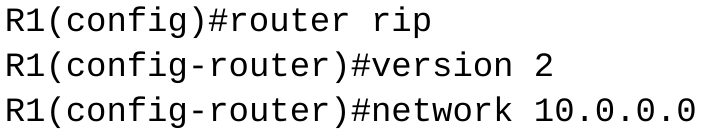
\includegraphics[width=0.7\linewidth]{img/img01}
	\end{figure}
	\begin{itemize}
		\item The ‘network’ command should reference a classful network. No subnet
		mask is specified.
	\end{itemize}
\end{frame}

\begin{frame}
	\frametitle{Auto-Summary}
	\begin{itemize}
		\item RIP will automatically summarise routes to the classful boundary by
default
		\item For example, 192.168.10.1/30 will be advertised as 192.168.10.0/24
		\item 172.16.10.1/30 will be advertised as 172.16.0.0/16
		\item This is almost never desirable
	\end{itemize}
	\begin{figure}
		\centering
		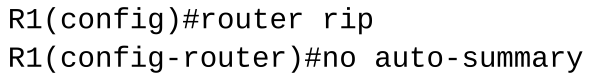
\includegraphics[width=0.7\linewidth]{img/img02}
	\end{figure}
\end{frame}

\begin{frame}
	\frametitle{Manual Summarization}
	\begin{itemize}
		\item Manual summarisation gives you control of exactly how you summarise
		\item The individual summarised routes are not advertised - only their summary
route
	\end{itemize}
	\begin{figure}
		\centering
		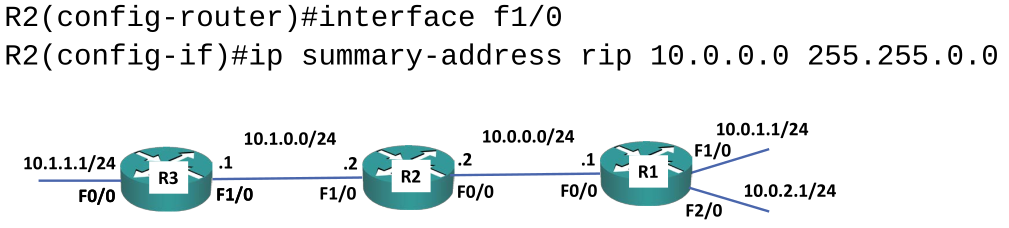
\includegraphics[width=\linewidth]{img/img03}
	\end{figure}
\end{frame}

\begin{frame}
	\frametitle{RIPv2 Verification – \\show ip protocols}
	\begin{figure}
		\centering
		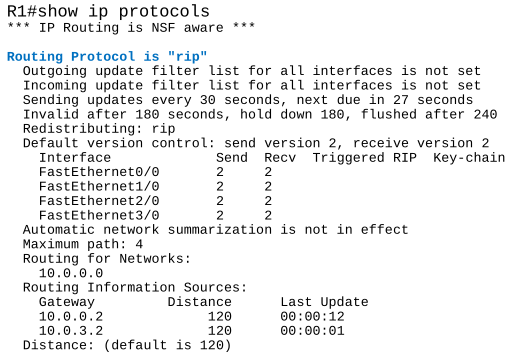
\includegraphics[width=0.8\linewidth]{img/img04}
	\end{figure}
\end{frame}

\begin{frame}
	\frametitle{RIPv2 Verification – \\show run | section rip}
	\begin{figure}
		\centering
		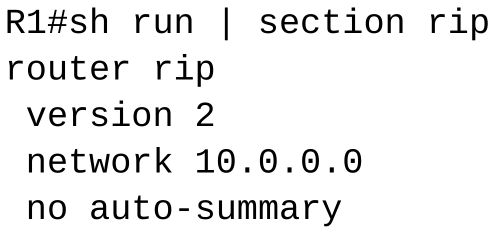
\includegraphics[width=0.8\linewidth]{img/img05}
	\end{figure}
\end{frame}

\begin{frame}
	\frametitle{RIPv2 Verification – \\show ip route}
	\begin{figure}
		\centering
		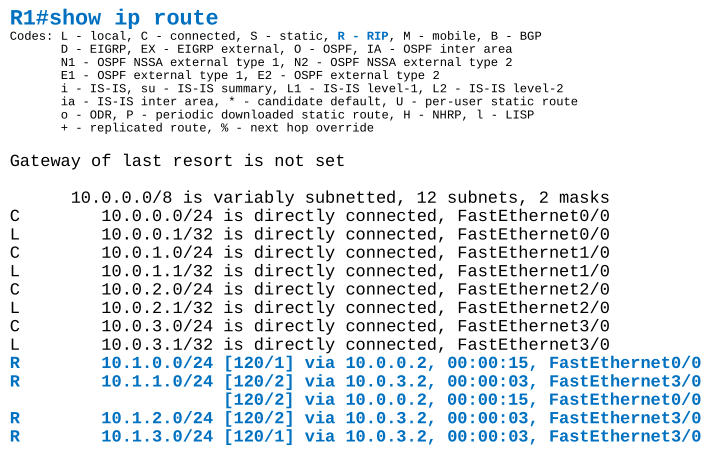
\includegraphics[width=0.8\linewidth]{img/img06}
	\end{figure}
\end{frame}

\begin{frame}
	\frametitle{RIPv2 Verification – \\show ip rip database}
	\begin{figure}
		\centering
		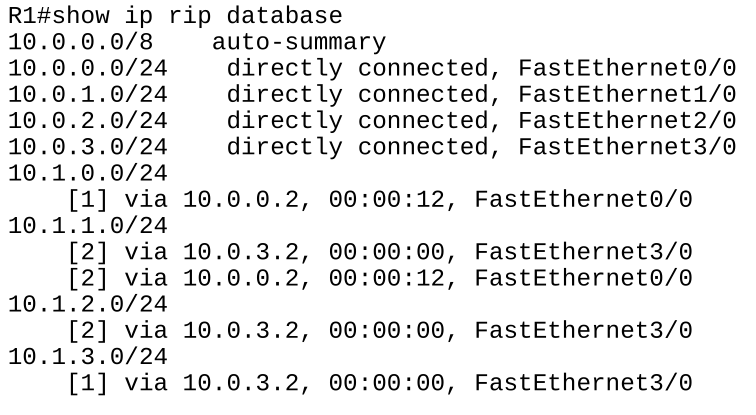
\includegraphics[width=0.8\linewidth]{img/img07}
	\end{figure}
\end{frame}

\begin{frame}
	\frametitle{Default Route Injection}
	\begin{figure}
		\centering
		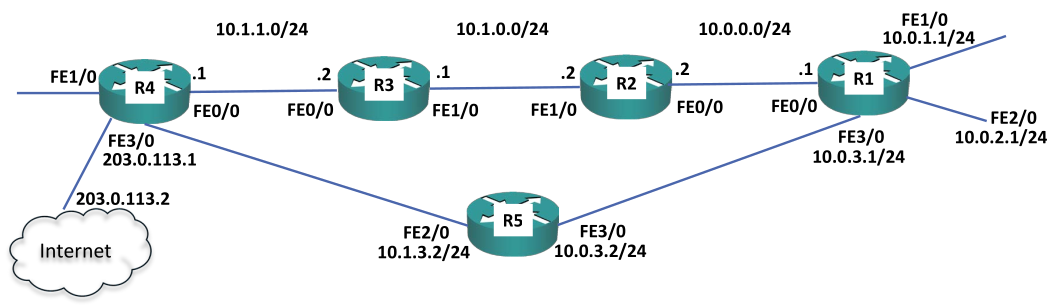
\includegraphics[width=\linewidth]{img/img08}
	\end{figure}
\end{frame}

\begin{frame}
	\frametitle{Default Route Injection}
	\begin{figure}
		\centering
		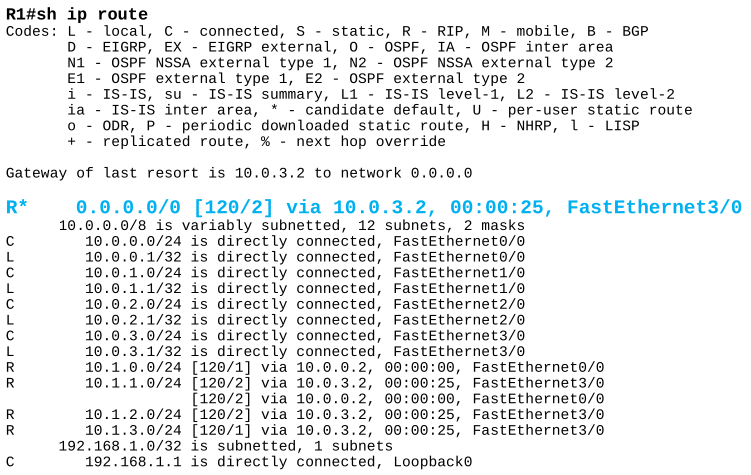
\includegraphics[width=\linewidth]{img/img09}
	\end{figure}
\end{frame}

\section{EIGRP - the Enhanced Interior Gateway Routing Protocol}

\begin{frame}
	\frametitle{EIGRP Characteristics}
	\begin{itemize}
		\item EIGRP (Enhanced Interior Gateway Routing Protocol) is an
Advanced Distance Vector routing protocol
		\item It supports large networks
		\item It has very fast convergence time
		\item It supports bounded updates where network topology change
updates are only sent to routers affected by the change
		\item Messages are sent using multicast
	\end{itemize}
\end{frame}

\begin{frame}{EIGRP Characteristics}
	\begin{itemize}
		\item EIGRP will automatically perform equal cost load balancing on
up to 4 paths by default
		\item This can be increased up to 16 paths
		\item EIGRP can also be configured to perform unequal cost load
balancing
	\end{itemize}
\end{frame}

\begin{frame}
	\frametitle{EIGRP Configuration – AS number}
	\begin{figure}
		\centering
		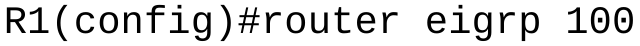
\includegraphics[width=0.6\linewidth]{img/img10}
	\end{figure}
	\begin{itemize}
		\item ‘100’ in this example is the Autonomous System (AS), meaning
an independent administrative domain. EIGRP routers need to
have the same Autonomous System number to peer with each
other.
	\end{itemize}
\end{frame}

\begin{frame}
	\frametitle{EIGRP Configuration - network}
	\begin{figure}
		\centering
		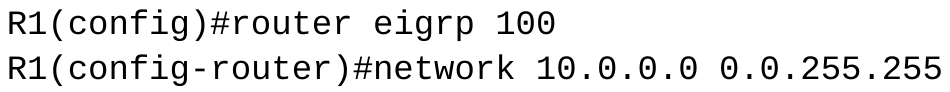
\includegraphics[width=\linewidth]{img/img11}
	\end{figure}
	\begin{itemize}
		\item The network command uses a wildcard mask which is the inverse of a
subnet mask.
		\item Subtract each octet in the subnet mask from 255 to calculate the
wildcard mask
		\item A subnet mask of 255.255.0.0 equals a wildcard mask of 0.0.255.255
		\item A subnet mask of 255.255.255.252 equals a wildcard mask of 0.0.0.3
	\end{itemize}
\end{frame}

\begin{frame}{EIGRP Configuration - network}
	\begin{figure}
		\centering
		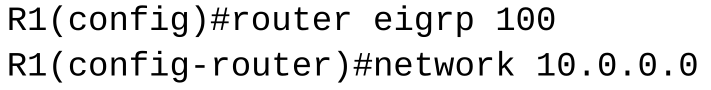
\includegraphics[width=0.8\linewidth]{img/img12}
	\end{figure}
	\begin{itemize}
		\item If you do not enter a wildcard mask, the command defaults to
using the classful boundary
		\item 0.255.255.255 for a Class A address
		\item 0.0.255.255 for a Class B address
		\item 0.0.0.255 for a Class C address
	\end{itemize}
\end{frame}

\begin{frame}{EIGRP Configuration - network}
	\begin{figure}
		\centering
		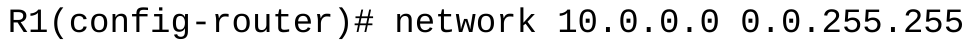
\includegraphics[width=\linewidth]{img/img13}
	\end{figure}
	\begin{itemize}
		\item The network command means:
		\begin{itemize}
			\item Look for interfaces with an IP address which falls within this
range.
			\item Enable EIGRP on those interfaces – send out and listen for
EIGRP hello messages, and peer with adjacent EIGRP
routers.
			\item Advertise the network and mask which is configured on
those interfaces.
		\end{itemize}
	\end{itemize}
\end{frame}

\begin{frame}
	\frametitle{EIGRP Configuration Example -\\ network}
	\begin{figure}
		\centering
		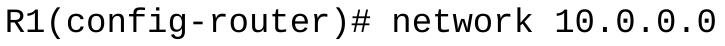
\includegraphics[width=0.8\linewidth]{img/img14}
	\end{figure}
	\begin{itemize}
		\item A default Class A wildcard of 0.255.255.255 will be used
		\item All interfaces fall within this range in our example
		\item EIGRP will be enabled on all interfaces and the router will peer with
adjacent EIGRP routers
		\item Networks advertised:
		\begin{multicols}{2}
			\begin{itemize}
				\item 10.1.0.0/24
				\item 10.0.1.0/24
				\item 10.0.2.0/24
				\item 10.0.0.0/8 is NOT advertised
			\end{itemize}
			\columnbreak
			\begin{figure}
				\centering
				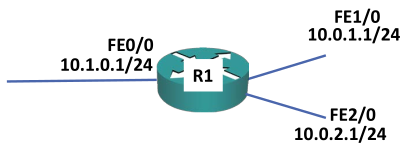
\includegraphics[width=\linewidth]{img/img15}
			\end{figure}
		\end{multicols}
	\end{itemize}
\end{frame}

\begin{frame}{EIGRP Configuration Example -\\ network}
	\begin{figure}
		\centering
		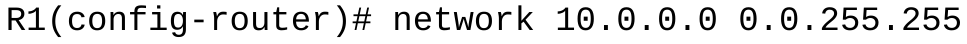
\includegraphics[width=\linewidth]{img/img16}
	\end{figure}
	\begin{itemize}
		\item Interface FE1/0 and FE2/0 fall within this range, FE0/0 does not
		\item EIGRP will be enabled on FE1/0 and FE2/0 and the router will peer with
adjacent EIGRP routers
		\item Networks advertised:
		\begin{multicols}{2}
			\begin{itemize}
				\item 10.0.1.0/24
				\item 10.0.2.0/24
				\item 10.1.0.0/24 is NOT advertised
				\item 10.0.0.0/16 is NOT advertised
			\end{itemize}
			\columnbreak
			\begin{figure}
				\centering
				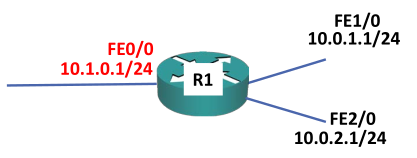
\includegraphics[width=\linewidth]{img/img17}
			\end{figure}
		\end{multicols}
	\end{itemize}
\end{frame}

\begin{frame}{EIGRP Configuration Example -\\ network}
	\begin{itemize}
		\item Two different configurations, same result:
		\item \texttt{R1(config-router)\# network 10.0.0.0}
		\item[]
		\item \texttt{R1(config-router)\# network 10.1.0.0 0.0.0.255}
		\item \texttt{R1(config-router)\# network 10.0.1.0 0.0.0.255}
		\item \texttt{R1(config-router)\# network 10.0.2.0 0.0.0.255}
	\end{itemize}
	\begin{figure}
		\centering
		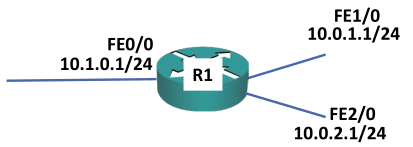
\includegraphics[width=0.6\linewidth]{img/img18}
	\end{figure}
\end{frame}

\begin{frame}{EIGRP Configuration Example -\\ network}
	\begin{itemize}
		\item Two different configurations, same result:
		\item \texttt{R1(config-router)\# network 10.0.0.0}
		\item[]
		\item \texttt{R1(config-router)\# network 10.1.0.1 0.0.0.0}
		\item \texttt{R1(config-router)\# network 10.0.1.1 0.0.0.0}
		\item \texttt{R1(config-router)\# network 10.0.2.1 0.0.0.0}
	\end{itemize}
	\begin{figure}
		\centering
		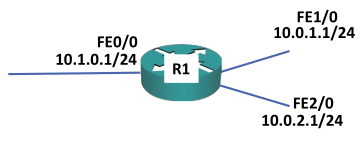
\includegraphics[width=0.6\linewidth]{img/img19}
	\end{figure}
\end{frame}

\begin{frame}
	\frametitle{EIGRP Router ID}
	\begin{itemize}
		\item EIGRP routers identify themselves using an EIGRP Router ID which is in
the form of an IP address.
		\item This will default to being the highest IP address of any loopback
interfaces configured on the router, or the highest other IP address if a
loopback does not exist.
		\item Loopback interfaces never go down so the Router ID will not change.
		\item You can also manually specify the Router ID.
		\item Best practice is to use a Loopback or manually set the Router ID.
	\end{itemize}
\end{frame}

\begin{frame}
	\frametitle{EIGRP Router ID – No Loopback}
	\begin{figure}
		\centering
		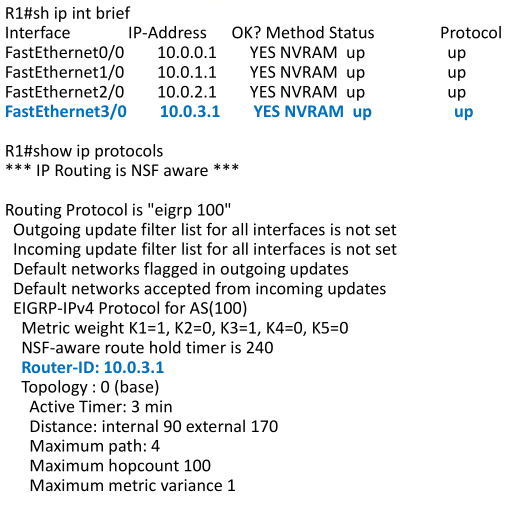
\includegraphics[width=0.6\linewidth]{img/img20}
	\end{figure}
\end{frame}

\begin{frame}
	\frametitle{EIGRP Router ID – Loopback}
	\begin{multicols}{2}
		\begin{figure}
			\centering
			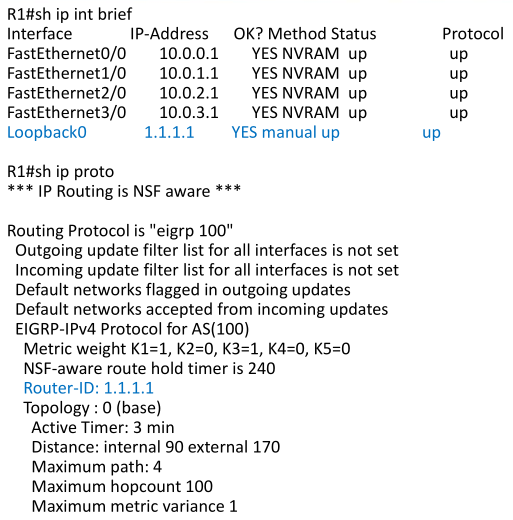
\includegraphics[width=\linewidth]{img/img21}
		\end{figure}
		\columnbreak
		\begin{itemize}
			\item If a loopback or higher IP
address is configured after
EIGRP has been set up, the
Router ID will change on
EIGRP process restart.
		\end{itemize}
	\end{multicols}	
\end{frame}

\begin{frame}
	\frametitle{EIGRP Router ID –\\ Manually Configured}
	\begin{figure}
		\centering
		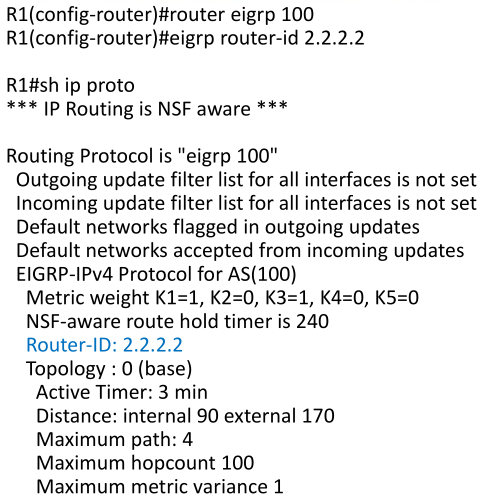
\includegraphics[height=0.8\textheight]{img/img22}
	\end{figure}
\end{frame}

\section{EIGRP Lab Demo}

\begin{frame}
	\frametitle{EIGRP Verification –\\ show run | section eigrp}
	\begin{figure}
		\centering
		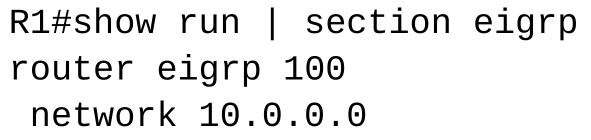
\includegraphics[width=0.7\linewidth]{img/img23}
	\end{figure}
\end{frame}

\begin{frame}
	\frametitle{EIGRP Verification –\\ show ip protocols}
	\begin{figure}
		\centering
		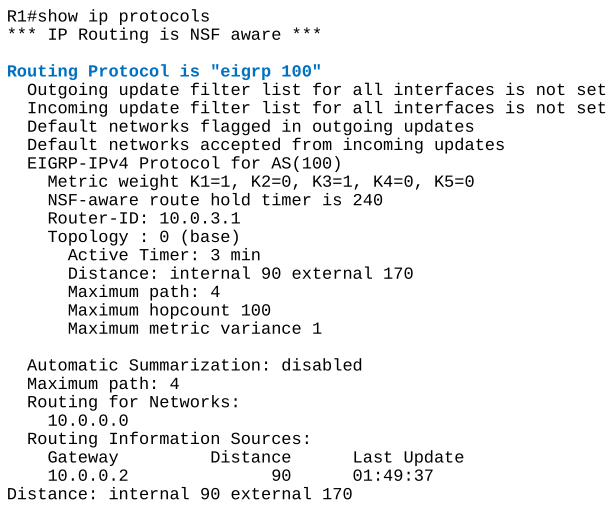
\includegraphics[height=0.8\textheight]{img/img24}
	\end{figure}
\end{frame}

\begin{frame}
	\frametitle{EIGRP Verification –\\ show ip eigrp interfaces}
	\begin{figure}
		\centering
		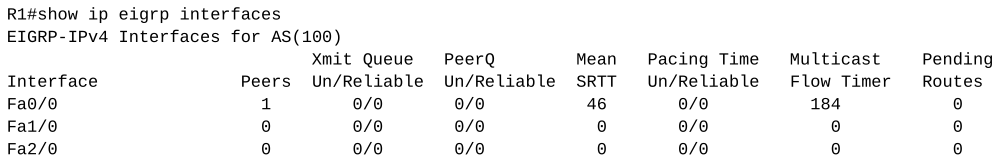
\includegraphics[width=\linewidth]{img/img25}
	\end{figure}
\end{frame}

\begin{frame}{EIGRP Verification –\\ show ip eigrp interfaces}
	\begin{figure}
		\centering
		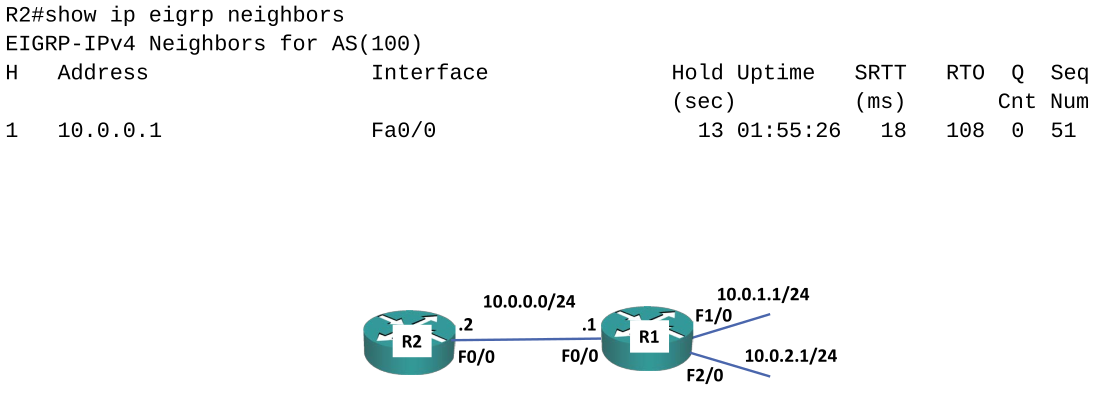
\includegraphics[width=\linewidth]{img/img26}
	\end{figure}
\end{frame}

\begin{frame}
	\frametitle{EIGRP Verification - show ip route}
	\begin{figure}
		\centering
		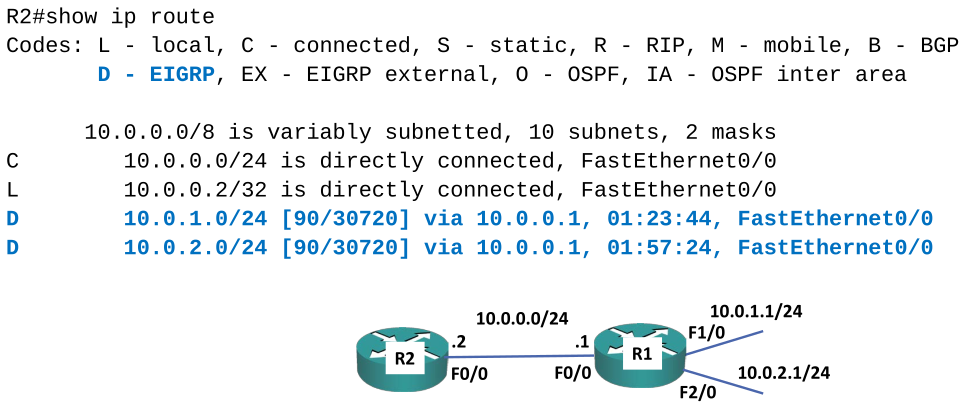
\includegraphics[width=\linewidth]{img/img27}
	\end{figure}
\end{frame}

\begin{frame}
	\frametitle{Lab}
	\begin{figure}
		\centering
		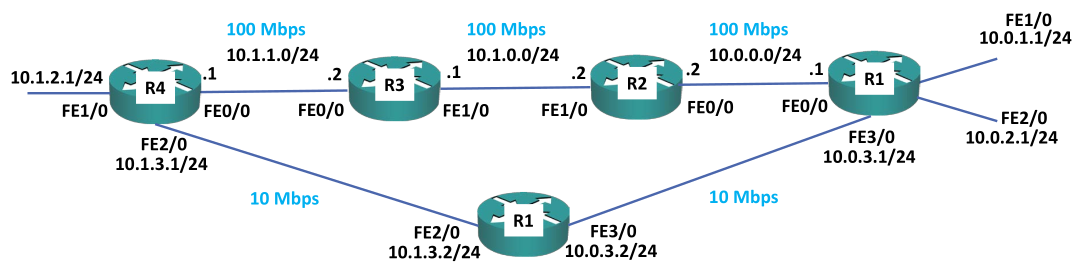
\includegraphics[width=\linewidth]{img/img28}
	\end{figure}
\end{frame}

\end{document}